\documentclass{article}

\usepackage{tabularx}

% https://tex.stackexchange.com/a/129100/125609, to draw the pico ampremeter
\usepackage{tikz}
\usetikzlibrary{arrows}
\usetikzlibrary{shapes}
\newcommand*\circled[1]{\tikz[baseline=(char.base)]{
		            \node[shape=circle,draw,inner sep=1pt] (char) {#1};}}

% NOTE: To put equations in their environment we need either `float` or
% `caption`.  We use float to put equations and other environments exactly
% where they appear in the code with the `H` placeholder, and for that we
% redefine the `equ` environment sort of twice, so this is a bit flaky but
% it works.
\usepackage{caption}
\DeclareCaptionType{equ}[][]
\captionsetup[equ]{name=נוסחא}
\usepackage{float}
\floatstyle{plain}
% https://www.overleaf.com/learn/latex/Positioning_of_Figures
\newfloat{equ}{H}{eq}[section]
\floatname{equ}{נוסחא}

\DeclareCaptionType{graph}[][]
\captionsetup[graph]{name=גרף }

% to includegraphics
\usepackage{graphicx}

% to fix itemize lists:
% https://tex.stackexchange.com/a/53453/125609
\usepackage{enumitem}
\setlist[itemize,1]{label={\fontfamily{cmr}\fontencoding{T1}\selectfont\textbullet}}

% Links
\usepackage{hyperref}
\hypersetup{colorlinks = true,
	citecolor = gray,
	linkcolor = red,
	citecolor = green,
	filecolor = magenta,
	urlcolor = cyan
}

\usepackage[version=4]{mhchem}

% To include plots by matplotlib
\usepackage{pgfplots}
\pgfplotsset{compat=newest}
% Note we use resizebox as explained here through out the document https://tex.stackexchange.com/a/582956/125609

% Language
\usepackage{polyglossia}
\setdefaultlanguage{hebrew}
\setotherlanguage{english}
\usepackage{hebrewcal}

% Fonts
\setmainfont{David CLM}
\setsansfont{Liberation Sans}
\setmonofont{Liberation Mono}
\newfontfamily\hebrewfont{David CLM}[Script=Hebrew]
\newfontfamily\hebrewfontsf{Liberation Serif}[Script=Hebrew]
\newfontfamily\hebrewfonttt{Liberation Mono}[Script=Hebrew]

\title{
אישור קיומן של רמות אנרגיה בדידות ומדידת אנרגיית היינון של אטום כספית
} 
\author{
שרה לחצר ודורון בכר \\
הפקולטה לפיזיקה, הטכניון - מכון טכנולוגי לישראל.
}
\date{\today}

\begin{document}
\maketitle

\begin{abstract}
	% TODO: Fill up
\end{abstract}

\section{מבוא}

לפי מודל אטום המימן, אלקטרונים באטום המימן מצויים ברמות אנרגיה בדידות. גם אטום
עם יותר אלקטרונים כגון אטום הכספית \ce{Hg}, אפשר למדל באופן דומה ולהראות
ניסיונית שגם לו רמות אנרגיה בדידות. רוב הניסויים שמראים זאת משתמשים בפוטונים
שנבלעים באטומים ומוסרים את האנרגיה שלהם ($h \ni$) תמורת עירור. אין הכרח
שהאנרגיה המעוררת תגיע מפוטון, אלא גם אלקטרון עם אנרגיה קינטית מתאימה אמור להיות
מסוגל לעורר אטומים בהתנגשות. באופן דומה, ניתן גם ליינן אטומים בהתנגשות ולא רק
לעורר אותם.

% TODO: Add explanations for our expectation out of the theory?

\section{מערכת הניסוי}

שרטוט סכמתי של המערכת ניתן לראות באיור \ref{fig:system-scheme-excitations}.
בכדי למדוד את אנרגיות היינון ואת אנרגיות העירור של אטומי כספית באמצעות התנגשות
עם אלקטרונים, השתמשנו במערכת בשדה חשמלי בין הקתודה והאנודה המסומנים באותיות $K$
ו-$A$. אלקטרונים אלו מואצים בתוך תא בו נמצאת הכספית, בפאזה גזית. בנוסף לאנודה
ולקתודה, השתמשנו באלקטרודה ($M$), כך שבינה לבין האנודה יש פוטנציאל כזה שדוחה את
האלקטרונים בהתאם למתח $V_r$. אם לא היתה כספית בתוך התא, אלא ואקום, היינו מצפים
שהאלקטרונים המואצים היו מגיעים לאלקטרודה $M$, במידה ו-$V_a \ge  V_r$, ונמדוד
זרם שלילי במד הזרם הרגיש המסומן ב.
\circled{pA}.

בהינתן אנרגיה קינטית מתאימה לאלקטרונים, התנגשותם באטומי כספית אמורה לגרום להם
לאבד את האנרגיה הקינטית שלהם ובכך לא להגיע לאלקטרודה $M$. לכן אנחנו מצפים
שבאנרגיה זו, נקבל זרם נמוך ב-
\circled{pA}.

גם כאשר האנרגיה הקינטית של האלקטרונים גדולה פי
$2$
מאנרגית העירור הראשונה, אנו מצפים שהאלקטרונים יעוררו שני אטומי כספית ונצפה בזרם נמוך גם כן - כי התנגשות של אלקטרון שכזה באטום כספית יעורר אותו ואחר כך לאלקטרון תישאר אנרגיה לעורר אטום כספית נוסף.

\begin{figure}[H]
	\centering
	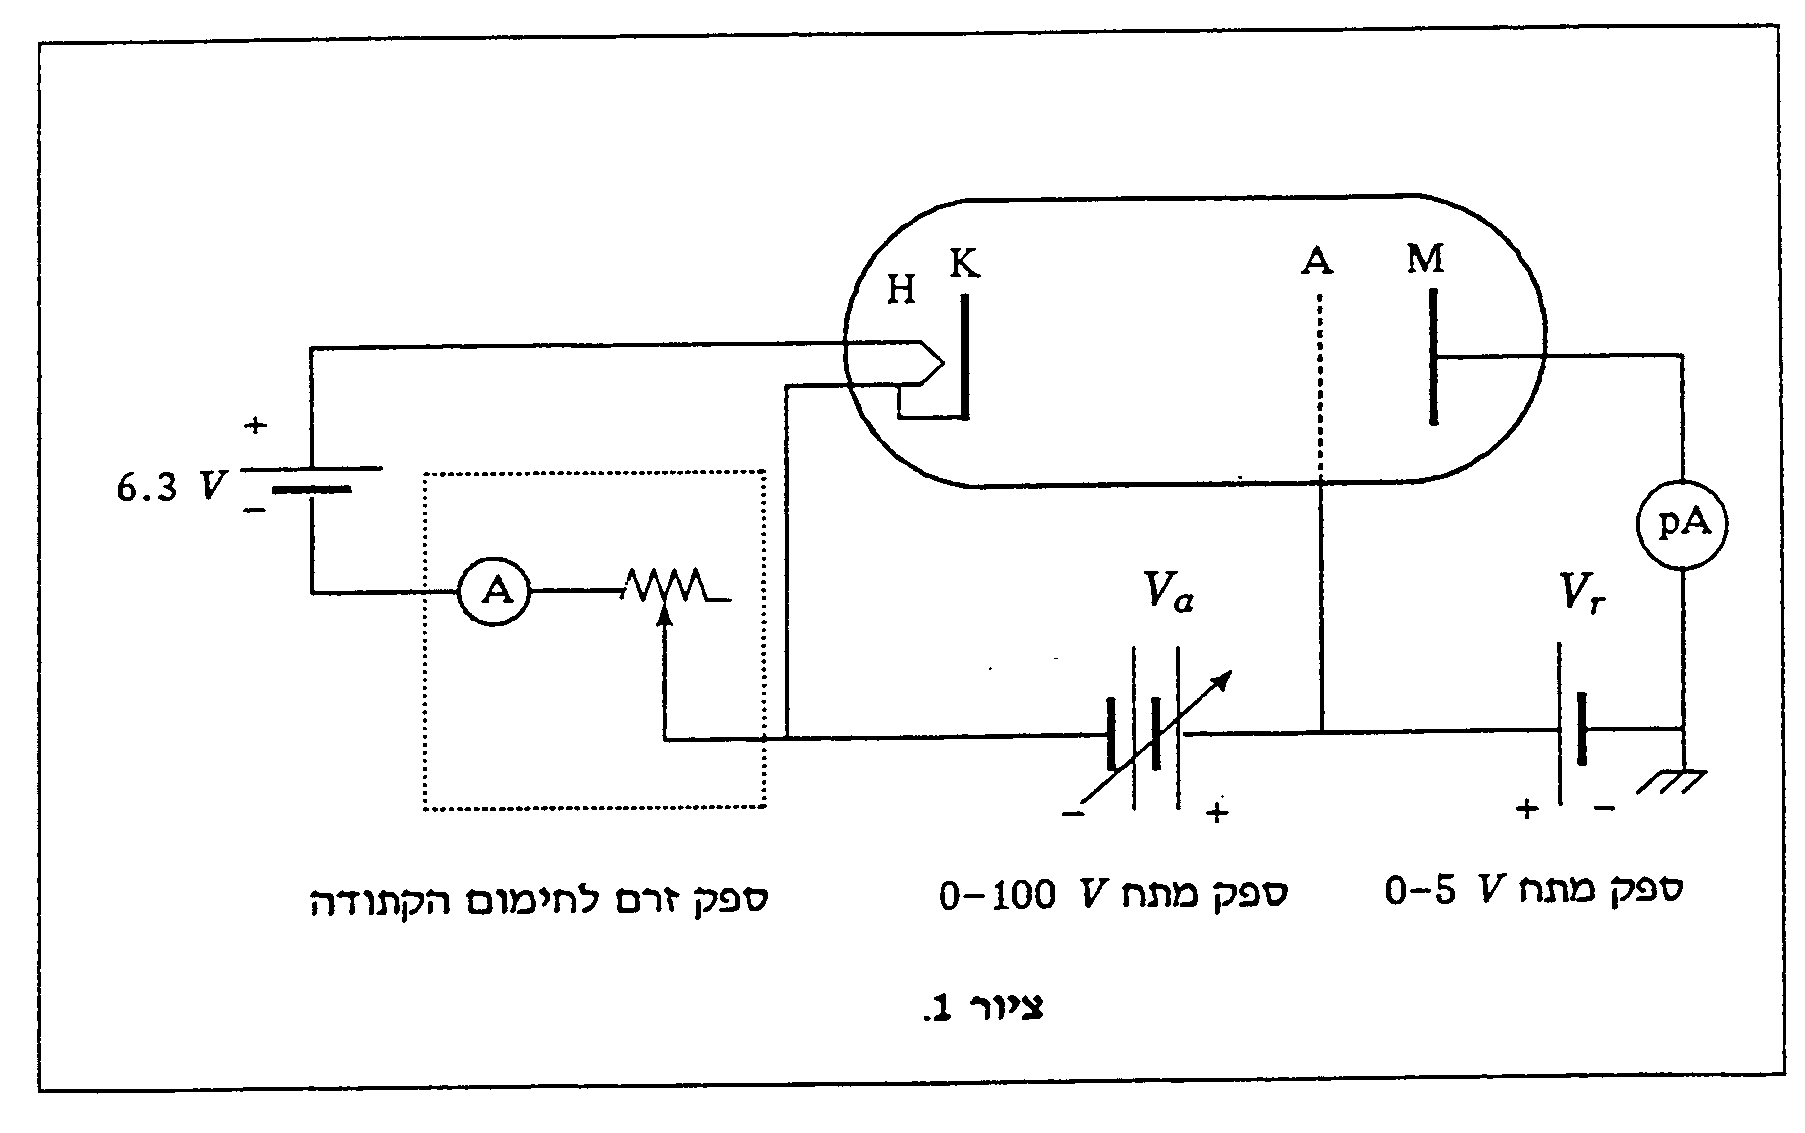
\includegraphics[width=\textwidth]{./system-scheme-excitations.png}
	\caption{שרטוט סכמתי של מערכת הניסוי - עבור עירורים}
	\label{fig:system-scheme-excitations}
\end{figure}



\section{תוצאות ודיון}
בחלקו הראשון של הניסוי מטרתנו הייתה לבחון את רמות האנרגיה הדיסקרטיות של אטום הכספית בעזרת המערכת של החלק הראשון המתוארת במבוא.
קיבענו את הטמפרטורה ל
$170 \deg C$,
ומדדנו את השינוי בזרם ההאצה כתלות במתח ההאצה.
חזרנו על הניסוי שלוש פעמים, ובכל פעם קיבלנו מקסימות של זרמים בהפרשים קבועים של המתח.
להלן מוצגת אחת מהמדידות שביצענו:

\section{סיכום}

% \section{מקורות}

% \printbibliography[heading=none]


\end{document}
